\documentclass[9pt,a4paper,]{extarticle}

\usepackage{f1000_styles}

\usepackage[pdfborder={0 0 0}]{hyperref}

\usepackage[numbers]{natbib}
\bibliographystyle{unsrtnat}


%% maxwidth is the original width if it is less than linewidth
%% otherwise use linewidth (to make sure the graphics do not exceed the margin)
\makeatletter
\def\maxwidth{ %
  \ifdim\Gin@nat@width>\linewidth
    \linewidth
  \else
    \Gin@nat@width
  \fi
}
\makeatother

\usepackage{color}
\usepackage{fancyvrb}
\newcommand{\VerbBar}{|}
\newcommand{\VERB}{\Verb[commandchars=\\\{\}]}
\DefineVerbatimEnvironment{Highlighting}{Verbatim}{commandchars=\\\{\}}
% Add ',fontsize=\small' for more characters per line
\usepackage{framed}
\definecolor{shadecolor}{RGB}{248,248,248}
\newenvironment{Shaded}{\begin{snugshade}}{\end{snugshade}}
\newcommand{\AlertTok}[1]{\textcolor[rgb]{0.94,0.16,0.16}{#1}}
\newcommand{\AnnotationTok}[1]{\textcolor[rgb]{0.56,0.35,0.01}{\textbf{\textit{#1}}}}
\newcommand{\AttributeTok}[1]{\textcolor[rgb]{0.77,0.63,0.00}{#1}}
\newcommand{\BaseNTok}[1]{\textcolor[rgb]{0.00,0.00,0.81}{#1}}
\newcommand{\BuiltInTok}[1]{#1}
\newcommand{\CharTok}[1]{\textcolor[rgb]{0.31,0.60,0.02}{#1}}
\newcommand{\CommentTok}[1]{\textcolor[rgb]{0.56,0.35,0.01}{\textit{#1}}}
\newcommand{\CommentVarTok}[1]{\textcolor[rgb]{0.56,0.35,0.01}{\textbf{\textit{#1}}}}
\newcommand{\ConstantTok}[1]{\textcolor[rgb]{0.00,0.00,0.00}{#1}}
\newcommand{\ControlFlowTok}[1]{\textcolor[rgb]{0.13,0.29,0.53}{\textbf{#1}}}
\newcommand{\DataTypeTok}[1]{\textcolor[rgb]{0.13,0.29,0.53}{#1}}
\newcommand{\DecValTok}[1]{\textcolor[rgb]{0.00,0.00,0.81}{#1}}
\newcommand{\DocumentationTok}[1]{\textcolor[rgb]{0.56,0.35,0.01}{\textbf{\textit{#1}}}}
\newcommand{\ErrorTok}[1]{\textcolor[rgb]{0.64,0.00,0.00}{\textbf{#1}}}
\newcommand{\ExtensionTok}[1]{#1}
\newcommand{\FloatTok}[1]{\textcolor[rgb]{0.00,0.00,0.81}{#1}}
\newcommand{\FunctionTok}[1]{\textcolor[rgb]{0.00,0.00,0.00}{#1}}
\newcommand{\ImportTok}[1]{#1}
\newcommand{\InformationTok}[1]{\textcolor[rgb]{0.56,0.35,0.01}{\textbf{\textit{#1}}}}
\newcommand{\KeywordTok}[1]{\textcolor[rgb]{0.13,0.29,0.53}{\textbf{#1}}}
\newcommand{\NormalTok}[1]{#1}
\newcommand{\OperatorTok}[1]{\textcolor[rgb]{0.81,0.36,0.00}{\textbf{#1}}}
\newcommand{\OtherTok}[1]{\textcolor[rgb]{0.56,0.35,0.01}{#1}}
\newcommand{\PreprocessorTok}[1]{\textcolor[rgb]{0.56,0.35,0.01}{\textit{#1}}}
\newcommand{\RegionMarkerTok}[1]{#1}
\newcommand{\SpecialCharTok}[1]{\textcolor[rgb]{0.00,0.00,0.00}{#1}}
\newcommand{\SpecialStringTok}[1]{\textcolor[rgb]{0.31,0.60,0.02}{#1}}
\newcommand{\StringTok}[1]{\textcolor[rgb]{0.31,0.60,0.02}{#1}}
\newcommand{\VariableTok}[1]{\textcolor[rgb]{0.00,0.00,0.00}{#1}}
\newcommand{\VerbatimStringTok}[1]{\textcolor[rgb]{0.31,0.60,0.02}{#1}}
\newcommand{\WarningTok}[1]{\textcolor[rgb]{0.56,0.35,0.01}{\textbf{\textit{#1}}}}

% disable code chunks background
%\renewenvironment{Shaded}{}{}

% disable section numbers
\setcounter{secnumdepth}{0}

%% added by MLS, this is not in the F1000 style by default %%

\hypersetup{unicode=true,
            pdftitle={target: An R Package to Predict Combined Function of Transcription Factors},
            pdfkeywords={transcription-factors; DNA-binding; gene-expression; r-package; bioconductor; workflow},
            pdfborder={0 0 0},
            breaklinks=true}

%% End added by MLS %%

\setlength{\parindent}{0pt}
\setlength{\parskip}{6pt plus 2pt minus 1pt}



\begin{document}
\pagestyle{front}

\title{target: An R Package to Predict Combined Function of Transcription Factors}

\author[1]{Mahmoud Ahmed}
\author[1]{Deok Ryong Kim}
\affil[1]{Department of Biochemistry and Convergence Medical Sciences and Institute of Health Sciences, Gyeongsang National University School of Medicine. Jinju, Korea}

\maketitle
\thispagestyle{front}

\begin{abstract}
Abstracts should be up to 300 words and provide a succinct summary of the article. Although the abstract should explain why the article might be interesting, care should be taken not to inappropriately over-emphasise the importance of the work described in the article. Citations should not be used in the abstract, and the use of abbreviations should be minimized.
\end{abstract}

\section*{Keywords}
transcription-factors; DNA-binding; gene-expression; r-package; bioconductor; workflow


\clearpage
\pagestyle{main}

\textbf{R version}: R version 3.6.1 (2019-07-05)

\textbf{Bioconductor version}: 3.9

\hypertarget{introduction}{%
\section{Introduction}\label{introduction}}

The introduction provides context as to why the software tool was developed and what need it addresses. It is good scholarly practice to mention previously developed tools that address similar needs, and why the current tool is needed.

\hypertarget{methods}{%
\section{Methods}\label{methods}}

\hypertarget{implementation}{%
\subsection{Implementation}\label{implementation}}

For software tool papers, this section should address how the tool works and any relevant technical details required for implementation of the tool by other developers.

\hypertarget{operation}{%
\subsection{Operation}\label{operation}}

This part of the methods should include the minimal system requirements needed to run the software and an overview of the workflow for the tool for users of the tool.

\hypertarget{use-cases}{%
\section{Use Cases }\label{use-cases}}

\begin{table}[htbp]
\caption{\label{tab:datasets} Expression and binding data of YY1 and YY2 in HeLa cells.}
\centering
\begin{tabledata}{@{}llll@{}}
\header GEO ID & Data Type & Design & Ref.\\
\row GSE14964 & Microarrays & YY\#-knockdown & \citet{Chen2010}\\
\row GSE31417 & ChIP-Seq & YY1 vs input & \citet{Michaud2013}\\
\row GSE96878 & ChIP-Seq & YY2 vs input & \citet{Wu2017d}\\
\end{tabledata}
\end{table}

Table \ref{tab:datasets}

\begin{Shaded}
\begin{Highlighting}[]
\CommentTok{# load required libraries}
\KeywordTok{library}\NormalTok{(tidyverse)}
\KeywordTok{library}\NormalTok{(reshape2)}
\KeywordTok{library}\NormalTok{(broom)}
\KeywordTok{library}\NormalTok{(cowplot)}
\KeywordTok{library}\NormalTok{(ggupset)}
\KeywordTok{library}\NormalTok{(seqLogo)}
\KeywordTok{library}\NormalTok{(ggplotify)}
\KeywordTok{library}\NormalTok{(rtracklayer)}
\KeywordTok{library}\NormalTok{(GenomicRanges)}
\KeywordTok{library}\NormalTok{(Biostrings)}
\KeywordTok{library}\NormalTok{(TxDb.Hsapiens.UCSC.hg19.knownGene)}
\KeywordTok{library}\NormalTok{(BSgenome.Hsapiens.UCSC.hg19)}
\KeywordTok{library}\NormalTok{(org.Hs.eg.db)}
\KeywordTok{library}\NormalTok{(BCRANK)}
\KeywordTok{library}\NormalTok{(target)}
\end{Highlighting}
\end{Shaded}

\hypertarget{preparing-the-binding-data}{%
\subsection{Preparing the binding data}\label{preparing-the-binding-data}}

\begin{Shaded}
\begin{Highlighting}[]
\CommentTok{# locate the peaks bed files}
\NormalTok{peak_files <-}\StringTok{ }\KeywordTok{c}\NormalTok{(}\DataTypeTok{YY1 =} \StringTok{'data/Oth.Utr.05.YY1.AllCell.bed'}\NormalTok{,}
                \DataTypeTok{YY2 =} \StringTok{'data/Oth.Utr.05.YY2.AllCell.bed'}\NormalTok{)}

\CommentTok{# load the peaks bed files as GRanges}
\NormalTok{peaks <-}\StringTok{ }\KeywordTok{map}\NormalTok{(peak_files, }\OperatorTok{~}\KeywordTok{GRanges}\NormalTok{(}\KeywordTok{import.bed}\NormalTok{(.x)))}
\end{Highlighting}
\end{Shaded}

\hypertarget{preparing-the-expression-data}{%
\subsection{Preparing the expression data}\label{preparing-the-expression-data}}

\begin{Shaded}
\begin{Highlighting}[]
\CommentTok{# locate the expression text files}
\NormalTok{expression_files <-}\StringTok{ }\KeywordTok{c}\NormalTok{(}\DataTypeTok{YY1 =} \StringTok{'data/DataSet_01_18.tsv'}\NormalTok{,}
                      \DataTypeTok{YY2 =} \StringTok{'data/DataSet_01_19.tsv'}\NormalTok{)}

\CommentTok{# load the expression text files}
\NormalTok{express <-}\StringTok{ }\KeywordTok{map}\NormalTok{(expression_files,}
               \OperatorTok{~}\KeywordTok{read_tsv}\NormalTok{(.x, }\DataTypeTok{col_names =} \OtherTok{FALSE}\NormalTok{) }\OperatorTok
\StringTok{                 }\NormalTok{dplyr}\OperatorTok{::}\KeywordTok{select}\NormalTok{(}\DecValTok{2}\NormalTok{,}\DecValTok{3}\NormalTok{, }\DecValTok{7}\NormalTok{, }\DecValTok{9}\NormalTok{) }\OperatorTok\StringTok{ }\CommentTok{#9}
\StringTok{                 }\KeywordTok{setNames}\NormalTok{(}\KeywordTok{c}\NormalTok{(}\StringTok{'tf'}\NormalTok{, }\StringTok{'gene'}\NormalTok{, }\StringTok{'fc'}\NormalTok{, }\StringTok{'pvalue'}\NormalTok{)) }\OperatorTok
\StringTok{                 }\KeywordTok{filter}\NormalTok{(tf }\OperatorTok\StringTok{ }\KeywordTok{c}\NormalTok{(}\StringTok{'YY1'}\NormalTok{, }\StringTok{'YY2'}\NormalTok{)) }\OperatorTok
\StringTok{                 }\KeywordTok{na.omit}\NormalTok{())}
\end{Highlighting}
\end{Shaded}

Figure \ref{fig:foldchange}

\begin{Shaded}
\begin{Highlighting}[]
\KeywordTok{par}\NormalTok{(}\DataTypeTok{mfrow =} \KeywordTok{c}\NormalTok{(}\DecValTok{1}\NormalTok{, }\DecValTok{3}\NormalTok{))}

\CommentTok{# volcano plot of YY1 knockdown}
\KeywordTok{plot}\NormalTok{(express}\OperatorTok{$}\NormalTok{YY1}\OperatorTok{$}\NormalTok{fc, }
     \OperatorTok{-}\KeywordTok{log10}\NormalTok{(express}\OperatorTok{$}\NormalTok{YY1}\OperatorTok{$}\NormalTok{pvalue),}
     \DataTypeTok{xlab =} \StringTok{'Fold-change (log_2)'}\NormalTok{,}
     \DataTypeTok{ylab =} \StringTok{'P-value (-log_10)'}\NormalTok{,}
     \DataTypeTok{xlim =} \KeywordTok{c}\NormalTok{(}\OperatorTok{-}\DecValTok{4}\NormalTok{, }\DecValTok{4}\NormalTok{), }\DataTypeTok{ylim =} \KeywordTok{c}\NormalTok{(}\DecValTok{0}\NormalTok{, }\DecValTok{6}\NormalTok{))}
\KeywordTok{title}\NormalTok{(}\StringTok{'(A)'}\NormalTok{)}

\CommentTok{# volcano plot of YY2 knockdown}
\KeywordTok{plot}\NormalTok{(express}\OperatorTok{$}\NormalTok{YY2}\OperatorTok{$}\NormalTok{fc, }
     \OperatorTok{-}\KeywordTok{log10}\NormalTok{(express}\OperatorTok{$}\NormalTok{YY2}\OperatorTok{$}\NormalTok{pvalue),}
     \DataTypeTok{xlab =} \StringTok{'Fold-change (log_2)'}\NormalTok{,}
     \DataTypeTok{ylab =} \StringTok{'P-value (-log_10)'}\NormalTok{,}
     \DataTypeTok{xlim =} \KeywordTok{c}\NormalTok{(}\OperatorTok{-}\DecValTok{4}\NormalTok{, }\DecValTok{4}\NormalTok{), }\DataTypeTok{ylim =} \KeywordTok{c}\NormalTok{(}\DecValTok{0}\NormalTok{, }\DecValTok{6}\NormalTok{))}
\KeywordTok{title}\NormalTok{(}\StringTok{'(B)'}\NormalTok{)}

\CommentTok{# plot fold-change of YY1 and YY2}
\KeywordTok{plot}\NormalTok{(express}\OperatorTok{$}\NormalTok{YY1}\OperatorTok{$}\NormalTok{fc[}\KeywordTok{order}\NormalTok{(express}\OperatorTok{$}\NormalTok{YY1}\OperatorTok{$}\NormalTok{gene)],}
\NormalTok{     express}\OperatorTok{$}\NormalTok{YY2}\OperatorTok{$}\NormalTok{fc[}\KeywordTok{order}\NormalTok{(express}\OperatorTok{$}\NormalTok{YY2}\OperatorTok{$}\NormalTok{gene)],}
     \DataTypeTok{xlab =} \StringTok{'YY1-knockdown (log_2)'}\NormalTok{,}
     \DataTypeTok{ylab =} \StringTok{'YY2-knockdown (log_2)'}\NormalTok{,}
     \DataTypeTok{xlim =} \KeywordTok{c}\NormalTok{(}\OperatorTok{-}\DecValTok{4}\NormalTok{, }\DecValTok{4}\NormalTok{), }\DataTypeTok{ylim =} \KeywordTok{c}\NormalTok{(}\OperatorTok{-}\DecValTok{4}\NormalTok{, }\DecValTok{4}\NormalTok{))}
\KeywordTok{title}\NormalTok{(}\StringTok{'(C)'}\NormalTok{)}
\end{Highlighting}
\end{Shaded}

\begin{figure}

{\centering \includegraphics[width=1\linewidth]{targetFlow_files/figure-latex/foldchange-1} 

}

\caption{Differential expression between factor knockdown and wild-type in HeLa cells.}\label{fig:foldchange}
\end{figure}

\hypertarget{preparing-genome-annotation}{%
\subsection{Preparing genome annotation}\label{preparing-genome-annotation}}

\begin{Shaded}
\begin{Highlighting}[]
\CommentTok{# load genome data}
\NormalTok{symbol_entrez <-}\StringTok{ }\KeywordTok{select}\NormalTok{(org.Hs.eg.db,}
                        \KeywordTok{unique}\NormalTok{(}\KeywordTok{c}\NormalTok{(express}\OperatorTok{$}\NormalTok{YY1}\OperatorTok{$}\NormalTok{gene)),}
                        \StringTok{'ENTREZID'}\NormalTok{,}
                        \StringTok{'SYMBOL'}\NormalTok{) }\OperatorTok
\StringTok{  }\KeywordTok{setNames}\NormalTok{(}\KeywordTok{c}\NormalTok{(}\StringTok{'gene'}\NormalTok{, }\StringTok{'gene_id'}\NormalTok{))}

\CommentTok{# format genome to join with express}
\NormalTok{genome <-}\StringTok{ }\KeywordTok{transcripts}\NormalTok{(TxDb.Hsapiens.UCSC.hg19.knownGene,}
                      \DataTypeTok{filter =} \KeywordTok{list}\NormalTok{(}\DataTypeTok{gene_id =}\NormalTok{ symbol_entrez}\OperatorTok{$}\NormalTok{gene_id),}
                      \DataTypeTok{columns =} \KeywordTok{c}\NormalTok{(}\StringTok{'tx_id'}\NormalTok{, }\StringTok{'tx_name'}\NormalTok{, }\StringTok{'gene_id'}\NormalTok{)) }\OperatorTok
\StringTok{  }\KeywordTok{promoters}\NormalTok{(}\DataTypeTok{upstream =} \DecValTok{100000}\NormalTok{) }\OperatorTok
\StringTok{  }\KeywordTok{as_tibble}\NormalTok{() }\OperatorTok
\StringTok{  }\KeywordTok{filter}\NormalTok{(}\KeywordTok{length}\NormalTok{(gene_id) }\OperatorTok{>}\StringTok{ }\DecValTok{1}\NormalTok{) }\OperatorTok
\StringTok{  }\KeywordTok{mutate}\NormalTok{(}\DataTypeTok{gene_id =} \KeywordTok{as.character}\NormalTok{(gene_id))}
\end{Highlighting}
\end{Shaded}

\begin{Shaded}
\begin{Highlighting}[]
\CommentTok{# make regions by merging the genome and express data}
\NormalTok{regions <-}\StringTok{ }\KeywordTok{map}\NormalTok{(express,}
               \OperatorTok{~}\KeywordTok{inner_join}\NormalTok{(genome, symbol_entrez) }\OperatorTok
\StringTok{                 }\KeywordTok{inner_join}\NormalTok{(.x) }\OperatorTok
\StringTok{                 }\KeywordTok{makeGRangesFromDataFrame}\NormalTok{(}\DataTypeTok{keep.extra.columns =} \OtherTok{TRUE}\NormalTok{))}
\end{Highlighting}
\end{Shaded}

\hypertarget{predicting-gene-targets-of-indiviual-factors}{%
\subsection{Predicting gene targets of indiviual factors}\label{predicting-gene-targets-of-indiviual-factors}}

\begin{Shaded}
\begin{Highlighting}[]
\CommentTok{# get associated peaks}
\NormalTok{ap <-}\StringTok{ }\KeywordTok{map2}\NormalTok{(peaks, regions,}
           \OperatorTok{~}\KeywordTok{associated_peaks}\NormalTok{(}\DataTypeTok{peaks=}\NormalTok{.x,}
                             \DataTypeTok{regions =}\NormalTok{ .y,}
                             \DataTypeTok{regions_col =} \StringTok{'tx_id'}\NormalTok{))}

\CommentTok{# get direct targets}
\NormalTok{dt <-}\StringTok{ }\KeywordTok{map2}\NormalTok{(peaks, regions,}
           \OperatorTok{~}\KeywordTok{direct_targets}\NormalTok{(}\DataTypeTok{peaks=}\NormalTok{.x,}
                           \DataTypeTok{regions =}\NormalTok{ .y,}
                           \DataTypeTok{regions_col =} \StringTok{'tx_id'}\NormalTok{,}
                           \DataTypeTok{stats_col =} \StringTok{'fc'}\NormalTok{))}
\end{Highlighting}
\end{Shaded}

Figure \ref{fig:functions}

\begin{Shaded}
\begin{Highlighting}[]
\KeywordTok{par}\NormalTok{(}\DataTypeTok{mfrow =} \KeywordTok{c}\NormalTok{(}\DecValTok{2}\NormalTok{, }\DecValTok{2}\NormalTok{))}

\CommentTok{# plot distance by score of associate peaks}
\KeywordTok{map2}\NormalTok{(ap, }\KeywordTok{c}\NormalTok{(}\StringTok{'(A)'}\NormalTok{, }\StringTok{'(B)'}\NormalTok{),}
     \OperatorTok{~}\NormalTok{\{}
       \KeywordTok{plot}\NormalTok{(.x}\OperatorTok{$}\NormalTok{distance,}
\NormalTok{            .x}\OperatorTok{$}\NormalTok{peak_score,}
            \DataTypeTok{xlab =} \StringTok{'Distance'}\NormalTok{,}
            \DataTypeTok{ylab =} \StringTok{'Peak Score'}\NormalTok{)}
       \KeywordTok{title}\NormalTok{(.y)}
\NormalTok{     \})}

\CommentTok{# make labels, colors and groups}
\NormalTok{labs <-}\StringTok{ }\KeywordTok{c}\NormalTok{(}\StringTok{'down'}\NormalTok{, }\StringTok{'none'}\NormalTok{, }\StringTok{'up'}\NormalTok{)}
\NormalTok{cols <-}\StringTok{ }\KeywordTok{c}\NormalTok{(}\StringTok{'green'}\NormalTok{, }\StringTok{'gray'}\NormalTok{, }\StringTok{'red'}\NormalTok{)}

\CommentTok{# make three groups by quantiles      }
\NormalTok{groups <-}\StringTok{ }\KeywordTok{map}\NormalTok{(dt,}
              \OperatorTok{~}\KeywordTok{cut}\NormalTok{(.x}\OperatorTok{$}\NormalTok{stat,}
                   \DataTypeTok{breaks =} \KeywordTok{quantile}\NormalTok{(.x}\OperatorTok{$}\NormalTok{stat, }\KeywordTok{c}\NormalTok{(}\DecValTok{0}\NormalTok{, }\FloatTok{.1}\NormalTok{, }\FloatTok{.9}\NormalTok{, }\DecValTok{1}\NormalTok{)),}
                   \DataTypeTok{labels =}\NormalTok{ labs))}

\CommentTok{# plot the group functions}
\KeywordTok{pmap}\NormalTok{(}\KeywordTok{list}\NormalTok{(dt, groups, }\KeywordTok{c}\NormalTok{(}\StringTok{'(C)'}\NormalTok{, }\StringTok{'(D)'}\NormalTok{)),}
    \ControlFlowTok{function}\NormalTok{(x, y, z) \{}
      \KeywordTok{plot_predictions}\NormalTok{(x}\OperatorTok{$}\NormalTok{score_rank,}
                       \DataTypeTok{group =}\NormalTok{ y,}
                       \DataTypeTok{colors =}\NormalTok{ cols,}
                       \DataTypeTok{labels =}\NormalTok{ labs,}
                       \DataTypeTok{xlab =} \StringTok{'Regulatory Potential'}\NormalTok{,}
                       \DataTypeTok{ylab =} \StringTok{'ECDF'}\NormalTok{)}
      
      \KeywordTok{title}\NormalTok{(z)}
\NormalTok{    \})}
\end{Highlighting}
\end{Shaded}

\begin{figure}

{\centering 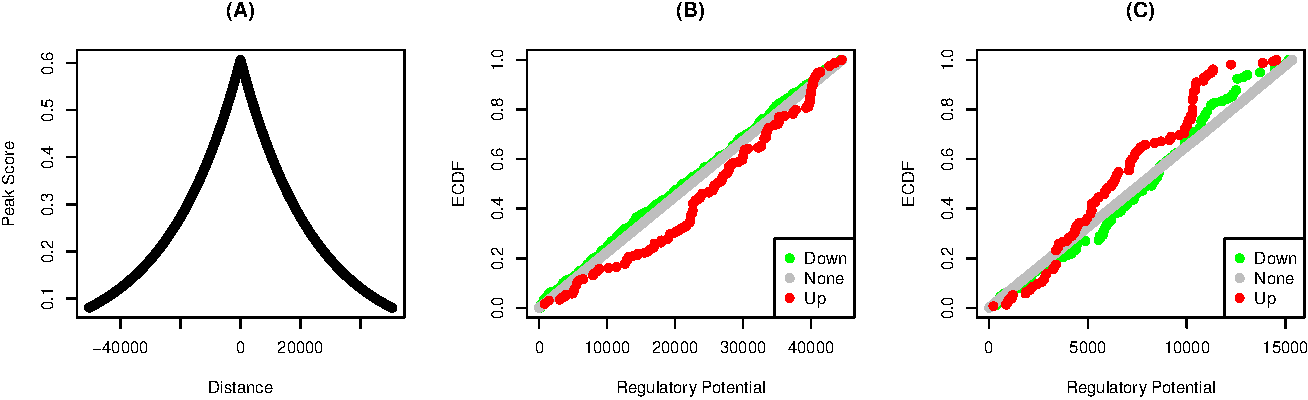
\includegraphics[width=1\linewidth]{targetFlow_files/figure-latex/functions-1} 

}

\caption{Predicted functions of YY1 and YY2 on their specific targets.}\label{fig:functions}
\end{figure}

\begin{Shaded}
\begin{Highlighting}[]
\CommentTok{# test individual factor functions}
\KeywordTok{map2}\NormalTok{(dt, groups,}
     \OperatorTok{~}\KeywordTok{test_predictions}\NormalTok{(.x}\OperatorTok{$}\NormalTok{rank,}
                       \DataTypeTok{group =}\NormalTok{ .y,}
                       \DataTypeTok{compare =} \KeywordTok{c}\NormalTok{(}\StringTok{'down'}\NormalTok{, }\StringTok{'up'}\NormalTok{)))}
\end{Highlighting}
\end{Shaded}

\begin{table}[htbp]
\caption{\label{tab:tests} Testing for statistical significance of the regulated gene groups.}
\centering
\begin{tabledata}{@{}lllll@{}}
\header Factor & Statistic & P.value & Method & Alternative\\
\row YY1 & 0.224 & 2.2e-16 & Two-sample KS test & two-sided\\
\row YY2 & 0.149 & 2.5e-15 & Two-sample KS test & two-sided\\
\end{tabledata}
\end{table}

Table \ref{tab:tests}

\hypertarget{predicting-the-shared-targets-of-two-factors}{%
\subsection{Predicting the shared targets of two factors}\label{predicting-the-shared-targets-of-two-factors}}

\begin{Shaded}
\begin{Highlighting}[]
\CommentTok{# merge and name peaks}
\NormalTok{common_peaks <-}\StringTok{ }\KeywordTok{reduce}\NormalTok{(}\KeywordTok{subsetByOverlaps}\NormalTok{(peaks}\OperatorTok{$}\NormalTok{YY1, peaks}\OperatorTok{$}\NormalTok{YY2))}
\NormalTok{common_peaks}\OperatorTok{$}\NormalTok{name <-}\StringTok{ }\KeywordTok{paste0}\NormalTok{(}\StringTok{'common_peak_'}\NormalTok{, }\DecValTok{1}\OperatorTok{:}\KeywordTok{length}\NormalTok{(common_peaks))}
\end{Highlighting}
\end{Shaded}

\begin{Shaded}
\begin{Highlighting}[]
\CommentTok{# bind express tables into one}
\NormalTok{both_express <-}\StringTok{ }\KeywordTok{bind_rows}\NormalTok{(express) }\OperatorTok
\StringTok{  }\KeywordTok{nest}\NormalTok{(fc, pvalue, }\DataTypeTok{.key =} \StringTok{'values_col'}\NormalTok{) }\OperatorTok
\StringTok{  }\KeywordTok{spread}\NormalTok{(tf, values_col) }\OperatorTok
\StringTok{  }\KeywordTok{unnest}\NormalTok{(YY1, YY2, }\DataTypeTok{.sep =} \StringTok{'_'}\NormalTok{)}

\CommentTok{# make regions using genome and expression data of both factors}
\NormalTok{both_regions <-}\StringTok{ }\KeywordTok{inner_join}\NormalTok{(genome, symbol_entrez) }\OperatorTok
\StringTok{  }\KeywordTok{inner_join}\NormalTok{(both_express) }\OperatorTok
\StringTok{  }\KeywordTok{makeGRangesFromDataFrame}\NormalTok{(}\DataTypeTok{keep.extra.columns =} \OtherTok{TRUE}\NormalTok{)}
\end{Highlighting}
\end{Shaded}

\begin{Shaded}
\begin{Highlighting}[]
\CommentTok{# get associated peaks with both factors}
\NormalTok{common_ap <-}\StringTok{ }\KeywordTok{associated_peaks}\NormalTok{(}\DataTypeTok{peaks =}\NormalTok{ common_peaks,}
                              \DataTypeTok{regions =}\NormalTok{ both_regions,}
                              \DataTypeTok{regions_col =} \StringTok{'tx_id'}\NormalTok{)}

\CommentTok{# get direct targets of both factors}
\NormalTok{common_dt <-}\StringTok{ }\KeywordTok{direct_targets}\NormalTok{(}\DataTypeTok{peaks =}\NormalTok{ common_peaks,}
                            \DataTypeTok{regions =}\NormalTok{ both_regions,}
                            \DataTypeTok{regions_col =} \StringTok{'tx_id'}\NormalTok{,}
                            \DataTypeTok{stats_col =} \KeywordTok{c}\NormalTok{(}\StringTok{'YY1_fc'}\NormalTok{, }\StringTok{'YY2_fc'}\NormalTok{))}
\end{Highlighting}
\end{Shaded}

Figure \ref{fig:function}

\begin{Shaded}
\begin{Highlighting}[]
\KeywordTok{par}\NormalTok{(}\DataTypeTok{mfrow =} \KeywordTok{c}\NormalTok{(}\DecValTok{1}\NormalTok{, }\DecValTok{2}\NormalTok{))}

\CommentTok{# plot distiace by score for associated peaks}
\KeywordTok{plot}\NormalTok{(common_ap}\OperatorTok{$}\NormalTok{distance,}
\NormalTok{     common_ap}\OperatorTok{$}\NormalTok{peak_score,}
     \DataTypeTok{xlab =} \StringTok{'Distance'}\NormalTok{,}
     \DataTypeTok{ylab =} \StringTok{'Peak Score'}\NormalTok{)}
\KeywordTok{title}\NormalTok{(}\StringTok{'(A)'}\NormalTok{)}

\CommentTok{# make labels, colors and gorups}
\NormalTok{labs <-}\StringTok{ }\KeywordTok{c}\NormalTok{(}\StringTok{'competitive'}\NormalTok{, }\StringTok{'none'}\NormalTok{, }\StringTok{'cooperative'}\NormalTok{)}
\NormalTok{cols <-}\StringTok{ }\KeywordTok{c}\NormalTok{(}\StringTok{'green'}\NormalTok{, }\StringTok{'gray'}\NormalTok{, }\StringTok{'red'}\NormalTok{)}

\CommentTok{# make three groups by quantiles      }
\NormalTok{common_groups <-}\StringTok{ }\KeywordTok{cut}\NormalTok{(common_dt}\OperatorTok{$}\NormalTok{stat,}
                     \DataTypeTok{breaks =} \KeywordTok{quantile}\NormalTok{(common_dt}\OperatorTok{$}\NormalTok{stat, }\KeywordTok{c}\NormalTok{(}\DecValTok{0}\NormalTok{, }\FloatTok{.1}\NormalTok{, }\FloatTok{.9}\NormalTok{, }\DecValTok{1}\NormalTok{)),}
                     \DataTypeTok{labels =}\NormalTok{ labs)}

\CommentTok{# plot predicted function}
\KeywordTok{plot_predictions}\NormalTok{(common_dt}\OperatorTok{$}\NormalTok{score_rank,}
                 \DataTypeTok{group =}\NormalTok{ common_groups,}
                 \DataTypeTok{colors =}\NormalTok{ cols,}
                 \DataTypeTok{labels =}\NormalTok{ labs,}
                 \DataTypeTok{xlab =} \StringTok{'Regulatory Potential'}\NormalTok{,}
                 \DataTypeTok{ylab =} \StringTok{'ECDF'}\NormalTok{)}
\KeywordTok{title}\NormalTok{(}\StringTok{'(B)'}\NormalTok{)}
\end{Highlighting}
\end{Shaded}

\begin{figure}

{\centering \includegraphics[width=1\linewidth]{targetFlow_files/figure-latex/function-1} 

}

\caption{Predicted function of YY1 and YY2 on their shared targets.}\label{fig:function}
\end{figure}

\begin{Shaded}
\begin{Highlighting}[]
\CommentTok{# test factors are cooperative}
\KeywordTok{test_predictions}\NormalTok{(common_dt}\OperatorTok{$}\NormalTok{score_rank,}
                 \DataTypeTok{group =}\NormalTok{ common_groups,}
                 \DataTypeTok{compare =} \KeywordTok{c}\NormalTok{(}\StringTok{'cooperative'}\NormalTok{, }\StringTok{'none'}\NormalTok{),}
                 \DataTypeTok{alternative =} \StringTok{'greater'}\NormalTok{)}

\CommentTok{# test factors are more cooperative than competitive}
\KeywordTok{test_predictions}\NormalTok{(common_dt}\OperatorTok{$}\NormalTok{score_rank,}
                 \DataTypeTok{group =}\NormalTok{ common_groups,}
                 \DataTypeTok{compare =} \KeywordTok{c}\NormalTok{(}\StringTok{'cooperative'}\NormalTok{, }\StringTok{'competitive'}\NormalTok{),}
                 \DataTypeTok{alternative =} \StringTok{'greater'}\NormalTok{)}
\end{Highlighting}
\end{Shaded}

\begin{table}[htbp]
\caption{\label{tab:test} Testing for statistical significance of combined functions of the two factors.}
\centering
\begin{tabledata}{@{}lllll@{}}
\header Compare & Satistic & P.value & Method & Alternative\\
\row Coop vs None & 0.168 & 1.5e-30 & KS test & The CDF of x lies above that of y\\
\row Coop vs Comp & 0.151 & 2.2e-16 & KS test & The CDF of x lies above that of y\\
\end{tabledata}
\end{table}

Table \ref{tab:test}

\hypertarget{binding-motif-analysis}{%
\subsection{Binding motif analysis}\label{binding-motif-analysis}}

\begin{Shaded}
\begin{Highlighting}[]
\CommentTok{# group peaks by their assigned targets}
\NormalTok{peak_groups <-}\StringTok{ }\KeywordTok{split}\NormalTok{(common_dt}\OperatorTok{$}\NormalTok{tx_id, common_groups)}

\CommentTok{# reorder peaks and get top n peaks}
\NormalTok{peak_groups <-}\StringTok{ }\KeywordTok{lapply}\NormalTok{(peak_groups, }\ControlFlowTok{function}\NormalTok{(x) \{}
    \CommentTok{# get peaks in x targets group}
\NormalTok{    p <-}\StringTok{ }\NormalTok{common_ap[common_ap}\OperatorTok{$}\NormalTok{assigned_region }\OperatorTok\StringTok{ }\KeywordTok{unique}\NormalTok{(x)]}
    
    \CommentTok{# order peaks by score}
\NormalTok{    p <-}\StringTok{ }\NormalTok{p[}\KeywordTok{order}\NormalTok{(p}\OperatorTok{$}\NormalTok{peak_score, }\DataTypeTok{decreasing =} \OtherTok{TRUE}\NormalTok{)]}
    
    \CommentTok{# get n top peaks}
    \CommentTok{#n <- length(p)}
\NormalTok{    n <-}\StringTok{ }\DecValTok{100}
\NormalTok{    p[}\DecValTok{1}\OperatorTok{:}\NormalTok{n]}
\NormalTok{\})}
\end{Highlighting}
\end{Shaded}

\begin{Shaded}
\begin{Highlighting}[]
\NormalTok{bcout <-}\StringTok{ }\KeywordTok{map}\NormalTok{(peak_groups[}\KeywordTok{c}\NormalTok{(}\StringTok{'competitive'}\NormalTok{, }\StringTok{'cooperative'}\NormalTok{)],}
             \OperatorTok{~}\NormalTok{\{}
               \CommentTok{# make a temporary file}
\NormalTok{               tmp_fasta <-}\StringTok{ }\KeywordTok{tempfile}\NormalTok{()}
               
               \CommentTok{# extract sequences of top peaks from the hg19 genome}
\NormalTok{               pseq <-}\StringTok{ }\KeywordTok{getSeq}\NormalTok{(BSgenome.Hsapiens.UCSC.hg19,}
                              \DataTypeTok{names =}\NormalTok{ .x)}
               
               \CommentTok{# write sequences to fasta file}
               \KeywordTok{writeXStringSet}\NormalTok{(pseq, tmp_fasta)}
               
               \CommentTok{# set random see}
               \KeywordTok{set.seed}\NormalTok{(}\DecValTok{123}\NormalTok{)}
                
               \CommentTok{# call bcrank with the fasta file}
               \KeywordTok{bcrank}\NormalTok{(tmp_fasta, }\DataTypeTok{silent =} \OtherTok{TRUE}\NormalTok{)}
\NormalTok{             \})}
\end{Highlighting}
\end{Shaded}

Figure \ref{fig:occurences}

\begin{Shaded}
\begin{Highlighting}[]
\KeywordTok{par}\NormalTok{(}\DataTypeTok{mfrow =} \KeywordTok{c}\NormalTok{(}\DecValTok{1}\NormalTok{, }\DecValTok{2}\NormalTok{))}

\CommentTok{# plot the occurences of consensus sequesnce in the regions}
\KeywordTok{map2}\NormalTok{(bcout, }\KeywordTok{c}\NormalTok{(}\StringTok{'(A)'}\NormalTok{, }\StringTok{'(B)'}\NormalTok{),}
     \OperatorTok{~}\NormalTok{\{}
       \KeywordTok{plot}\NormalTok{(}\KeywordTok{toptable}\NormalTok{(.x, }\DecValTok{1}\NormalTok{))}
       \KeywordTok{title}\NormalTok{(.y)}
\NormalTok{     \})}
\end{Highlighting}
\end{Shaded}

\begin{figure}

{\centering \includegraphics[width=1\linewidth]{targetFlow_files/figure-latex/occurences-1} 

}

\caption{Occurences of consensus sequences in the ranked regions.}\label{fig:occurences}
\end{figure}

\begin{verbatim}
## $competitive
## NULL
## 
## $cooperative
## NULL
\end{verbatim}

Figure \ref{fig:motifs}

\begin{Shaded}
\begin{Highlighting}[]
\KeywordTok{map}\NormalTok{(bcout, }\KeywordTok{c}\NormalTok{(}\StringTok{'(A)'}\NormalTok{, }\StringTok{'(B)'}\NormalTok{),}
    \OperatorTok{~}\NormalTok{\{}
      \KeywordTok{seqLogo}\NormalTok{(}\KeywordTok{pwm}\NormalTok{(}\KeywordTok{toptable}\NormalTok{(.x, }\DecValTok{1}\NormalTok{)))}
      \KeywordTok{title}\NormalTok{(.y)}
\NormalTok{    \})}
\end{Highlighting}
\end{Shaded}

\begin{figure}

{\centering \includegraphics[width=1\linewidth]{targetFlow_files/figure-latex/motifs-1} 

}

\caption{Predicted motifs of the cooperative and competitive binding sites.}\label{fig:motifs}
\end{figure}

\hypertarget{summary}{%
\section{Summary }\label{summary}}

This section is required if the paper does not include novel data or analyses. It allows authors to briefly summarize the key points from the article.

\hypertarget{software-availability}{%
\section{Software availability}\label{software-availability}}

This section will be generated by the Editorial Office before publication. Authors are asked to provide some initial information to assist the Editorial Office, as detailed below.

\begin{enumerate}
\def\labelenumi{\arabic{enumi}.}
\item
  URL link to where the software can be downloaded from or used by a non-coder (AUTHOR TO PROVIDE; optional)
\item
  URL link to the author's version control system repository containing the source code (AUTHOR TO PROVIDE; required)
\item
  Link to source code as at time of publication (\emph{F1000Research} TO GENERATE)
\item
  Link to archived source code as at time of publication (\emph{F1000Research} TO GENERATE)
\item
  Software license (AUTHOR TO PROVIDE; required)
\end{enumerate}

\hypertarget{author-information}{%
\section{Author information}\label{author-information}}

In order to give appropriate credit to each author of an article, the individual contributions of each author to the manuscript should be detailed in this section. We recommend using author initials and then stating briefly how they contributed.

\hypertarget{competing-interests}{%
\section{Competing interests}\label{competing-interests}}

All financial, personal, or professional competing interests for any of the authors that could be construed to unduly influence the content of the article must be disclosed and will be displayed alongside the article. If there are no relevant competing interests to declare, please add the following: `No competing interests were disclosed'.

\hypertarget{grant-information}{%
\section{Grant information}\label{grant-information}}

Please state who funded the work discussed in this article, whether it is your employer, a grant funder etc. Please do not list funding that you have that is not relevant to this specific piece of research. For each funder, please state the funder's name, the grant number where applicable, and the individual to whom the grant was assigned. If your work was not funded by any grants, please include the line: `The author(s) declared that no grants were involved in supporting this work.'

\hypertarget{acknowledgments}{%
\section{Acknowledgments}\label{acknowledgments}}

This section should acknowledge anyone who contributed to the research or the article but who does not qualify as an author based on the criteria provided earlier (e.g.~someone or an organization that provided writing assistance). Please state how they contributed; authors should obtain permission to acknowledge from all those mentioned in the Acknowledgments section.

Please do not list grant funding in this section.

{\small\bibliography{references.bib}}

\end{document}
